\documentclass[12pt, a4paper,oneside, openany]{book}
%fuente12pt,tamaño carta,una cara,quitar hojas en blanco,tipo libro
\usepackage[utf8]{inputenc} %fuente Unicode
%\usepackage[margin=-0cm]{geometry} %margen
\usepackage{graphicx} %uso de imagenes
\usepackage{multicol} %uso de multicolumnas
\usepackage{multirow} %multi celdas
\usepackage{lastpage} %n.total de paginas
\usepackage{colortbl} %columnas de color
\usepackage{tikz, tikz-3dplot} %figuras
\usepackage{tkz-euclide}
\usepackage{adjustbox} %manejo de margenes
\usepackage[spanish]{babel} %lenguaje español
\usepackage[document]{ragged2e} %alineacion
\usepackage[T1]{fontenc} %codificacion fuente
\usepackage{enumerate} %viñeta numeros
\usepackage{palatino} %fuente
\usepackage[colorlinks,linkcolor=myblue,citecolor=mygreen]{hyperref} %link personalizado
%-----------------------------------------------------------------
\definecolor{myblue}{HTML}{2D74B5} %color de titulos y subtitulos
%-----------------------------------------------------------------
\graphicspath{ {img/} } %localizacion de carpeta con imagenes
\renewcommand{\baselinestretch}{1.2} %espacio entre parrafos

%\AtBeginDocument{\AtBeginShipoutNext{\AtBeginShipoutDiscard}}
%elimina paginas adicionales que se agregan con el uso de hyperref
\usepackage{multirow} %multi celdas en tablas
\usepackage{longtable} %tablas multipagina
\usepackage{caption} %ajuste de tablas, figuras
\usepackage{color} %colores de texto
\usepackage{wrapfig} %rodear imagenes
\usepackage{booktabs, multirow} %bordes y rangos
\usepackage{titlesec} %titulos personalizados
\usepackage{eso-pic,picture} %imagenes con texto
\usepackage{nomencl} %simbolos de nomenclatura
\usepackage{lipsum} %crea texto default
\makenomenclature %tamaño nomenclatura
%\usepackage{showframe} %muestra el margen de las pg
%-----------------------------------------------------------------
%codigo del borde
\AddToShipoutPicture{%
\setlength\fboxsep{1pt}%
\put(24pt,24pt){\framebox(19.3066cm,28.0066cm)[lb]{}}%
}

%margenes
\usepackage{geometry}
\newgeometry{
        top=0.001in,
        bottom=3.2in,
        outer=0.55in,  %izquierda
        inner=0.55in, %derecha
        }
%-----------------------------------------------------------------
\usepackage{fancyhdr}%uso de encabezado y pie personalizado
\pagestyle{fancy}

\setlength{\headheight}{160pt}%ubicacion de caja de encabezado

\titlespacing{\chapter}{0pt}{-42pt}{0.5cm}%config capitulos, espacio de chapter
\titleformat{\chapter}[display]
{\sffamily\color{myblue}} {
    {\normalfont\color{myblue}\Large}
        \hspace{0pt}
            {\setlength\fboxsep{0pt}
                \colorbox{myblue}{
                }
            }
    }
{0 pt}
{\titlerule[0pt]\LARGE\sffamily}

%%%%%%%%%%%%%%%%%%%%%%%%%%%%%%%%%%%%%%%%%%%%%%%%%%%%%%%%%%%%%%%%%%%%%%%
\fancyhf{}%Declaración de encabezado
\pagestyle{fancy}
\fancypagestyle{plain}{}%encabezado general

\begin{document}%inicio de documento

\lhead{

\begin{minipage}{0.1\textwidth}
\scalebox{1}[1.2]{
\begin{tabular}{|m{2cm}|m{10.8cm}|m{1.0cm}|m{1.0cm}|m{1.0cm}| }

\hline

\multirow{3}{2cm}{\centering
\includegraphics[width=0.88\textwidth]{tjacdmx_logo.png}}
& \footnotesize\centering\bf\sffamily{TRIBUNAL DE JUSTICIA ADMINISTRATIVA DE TABASCO}
& \footnotesize\bf\sffamily{Día}
& \footnotesize\bf\sffamily{Mes}
&\footnotesize\bf\sffamily{Año}
\\ \cline{2-5}

& \centering\bf\footnotesize\sffamily{DIRECCIÓN GENERAL DE ADMINISTRACIÓN}
& \footnotesize\bf\sffamily{27}
& \footnotesize\bf\sffamily{02}
& \footnotesize\bf\sffamily{2023}
\\ \cline{2-5}

& \centering\bf\footnotesize\sffamily{DIRECCIÓN DE INFORMÁTICA}
& \multicolumn{3}{ |c| }{\bf\footnotesize\sffamily{Versión: 001 }}
\\ \cline{2-5}

&
\centering\bf\footnotesize\sffamily{MANUAL DE USUARIO}
& \multicolumn{3}{ |c| } {\bf\footnotesize\sffamily{Página \thepage~de\ \pageref{LastPage}}}
\\ \hline

\end{tabular}}
\end{minipage}

}
%-----------------------------------------------------------------

\centerline{
\includegraphics[width=0.8\textwidth]{tjacdmx_logo.png}}%imagen de logo en portada
%titulo de portada

\vspace{1cm}%espacio
%-----------------------------------------------------------------
\begin{flushright}%alineación a la derecha

\newcommand{\ProjectTitle}

\vspace{0cm}
%titulo en portada
{\color{myblue}{\sffamily\large\bf\sffamily
ACTUARIA V3.0 \\
ADMINISTRACIÓN\\
\vspace{0.3cm}
MANUAL DE USUARIO\\
\vspace{0.2cm}
DIRECCIÓN DE INFORMÁTICA}
}

\end{flushright}
%-----------------------------------------------------------------
%pie de todas las paginas
\cfoot[]{
{\tiny
\scalebox{1}[1.2]{%tamaño de celdas
\centering\begin{tabular}{|m{4cm}|m{4.0cm}|m{4.0cm}|m{4.0cm}| }

\hline

\centering\sffamily IDENTIFICACIÓN
& \centering\sffamily ELABORÓ
&  \centering\sffamily REVISÓ
& AUTORIZÓ
\\
\hline

\centering\sffamily TJACDMX DI MANUAL USUARIO
&  \centering\sffamily Dirección de Informática
&  \centering\sffamily Dirección de Informática
&  Comité Técnico Interno de Administración de Documentos del
TJACDMX en su sesión...
\\
\hline
\end{tabular}}

}}
%-----------------------------------------------------------------


\renewcommand{\headrulewidth}{0pt}%sin linea por default
\begin{quote}%alineacion de texto

\tableofcontents

\chapter{\large{Objetivo}}\label{chap:objetivo}
Con la finalidad de ofrecer a los servidores públicos del Tribunal de Justicia Administrativa de Tabasco
una herramienta que facilite la operación de los apartados que integran el módulo
de «Actuaría v 3.0», se elaboró el presente Manual.

\chapter{\large{¿Cómo ingresar a Actuaría v3.0?}}\label{chap:ingreso}

1.Ingresaremos al Sistema con el siguiente link:

\begin{center}
\href{https://sidj.tjacdmx.gob.mx}{https://sidj.tjacdmx.gob.mx}
\end{center}

2.Nos ubicaremos en el menú y daremos clic en  {\bf{
<<Actuaria v3.0>> }}

\begin{center}
    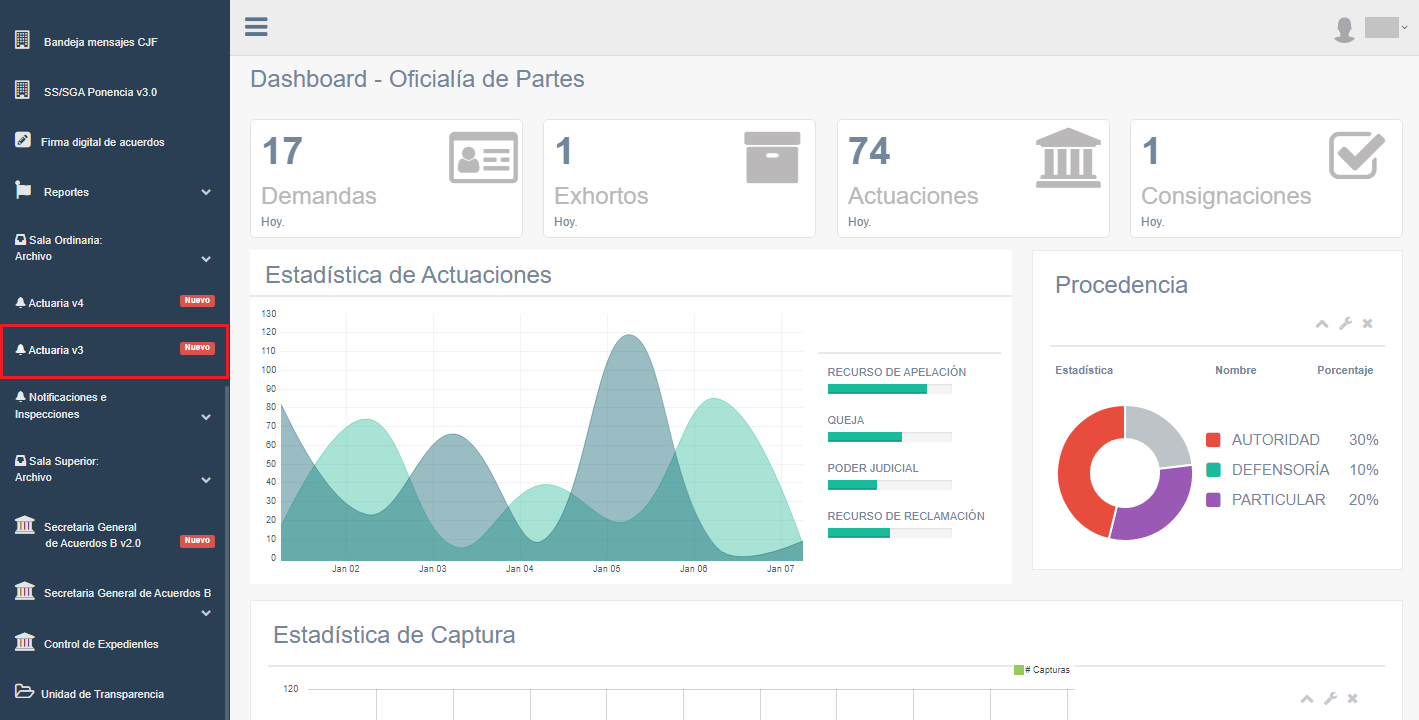
\includegraphics[width=0.88\columnwidth]{inicioAc.png}
\end{center}

\chapter{\large{Administración -  Plantillas v1.0.1}}\label{}

En esta sección de Administración de plantillas podrás realizar las siguientes actividades:

\begin{itemize}
    \item Búsqueda de carpeta.
    \item Añadir carpeta.
    \item Agregar permisos.
    \item Información.
    \item Editar.
    \item Eliminar.
    \item Registro de carpeta de plantillas.
\end{itemize}


{\Huge{\color{myblue} \section{¿Cómo buscar carpeta?}\label{sec:24}}}
Para hacer la búsqueda de una carpeta, ingresaremos el nombre en la siguiente pantalla y daremos clic en el botón {\bf{ <<Buscar>>}}

\begin{center}
    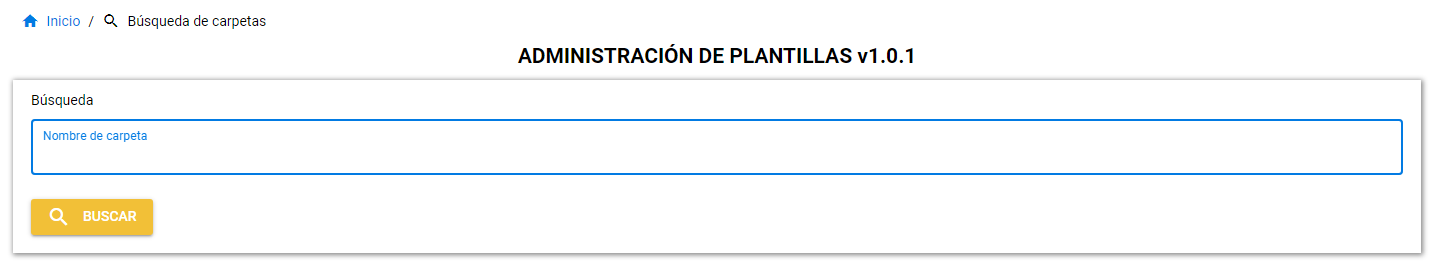
\includegraphics[width=0.90\columnwidth]{buscarc.png}
\end{center}

{\Huge{\color{myblue} \section{¿Cómo agregar una carpeta?}\label{sec:25}}}

\begin{center}
    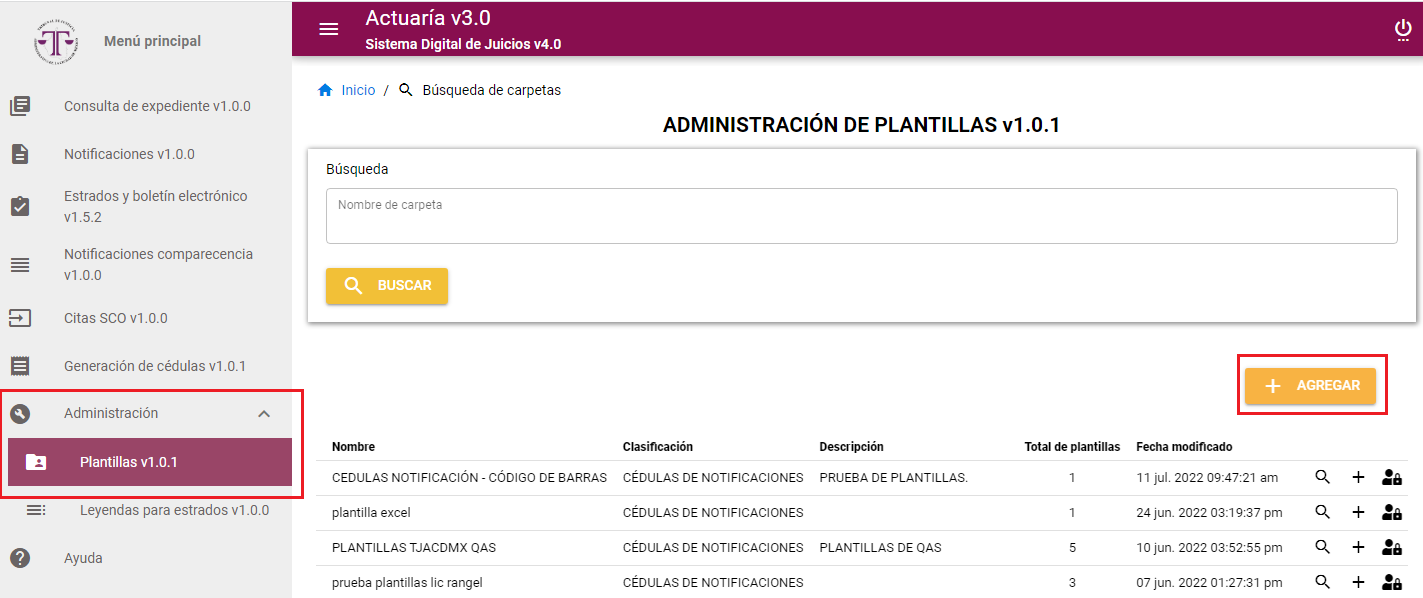
\includegraphics[width=0.90\columnwidth]{plantilla3.png}
\end{center}

Para añadir una plantilla nos ubicaremos en {\bf{ <<Plantillas v1.0.1>>}}
y daremos clic en el botón {\bf{ << + AGREGAR>>}} \\
Automáticamente nos aparecerá la siguiente pantalla:

\begin{center}
    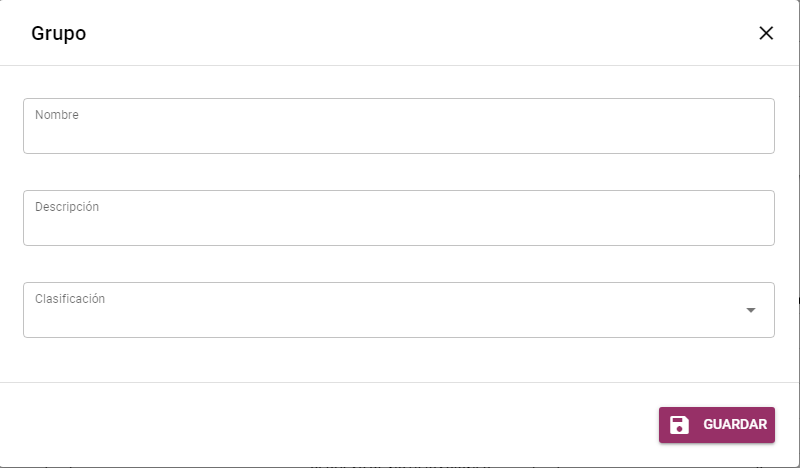
\includegraphics[width=0.50\columnwidth]{GRUPO.png}
\end{center}

Ingresaremos los siguientes datos:
\begin{itemize}
    \item Nombre
    \item Descripción
    \item Clasificación
\end{itemize}

Y daremos clic en el botón {\bf{ <<GUARDAR>>}}

{\Huge{\color{myblue} \section{Iconos}\label{sec:26}}}
\begin{center}
    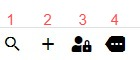
\includegraphics[width=0.30\columnwidth]{iconos.jpeg}
\end{center}
Podemos realizar las siguientes acciones:

\begin{enumerate}[(1)]
    \item Consultar
    \item Añadir plantilla +
    \item Agregar permisos
    \item Mas 
    \begin{itemize}
        \item Información.
        \item Editar.
        \item Eliminar
    \end{itemize}
\end{enumerate}

{\Huge{\color{myblue} \section{Consultar}\label{sec:27}}}

Para consultar carpeta de plantillas dar clic  en el icono     
\includegraphics[width=0.05\columnwidth]{lupa.png}
y nos mostrará la siguiente pantalla.

Dónde podemos observar:


{\color{myblue}
\begin{itemize}
    \item Nombre de carpeta.
    \item Clasificación.
    \item Propietario (Creador de la carpeta).
    \item Fecha de creación.
    \item Listado de las plantillas creadas
\end{itemize}
}
\begin{center}
    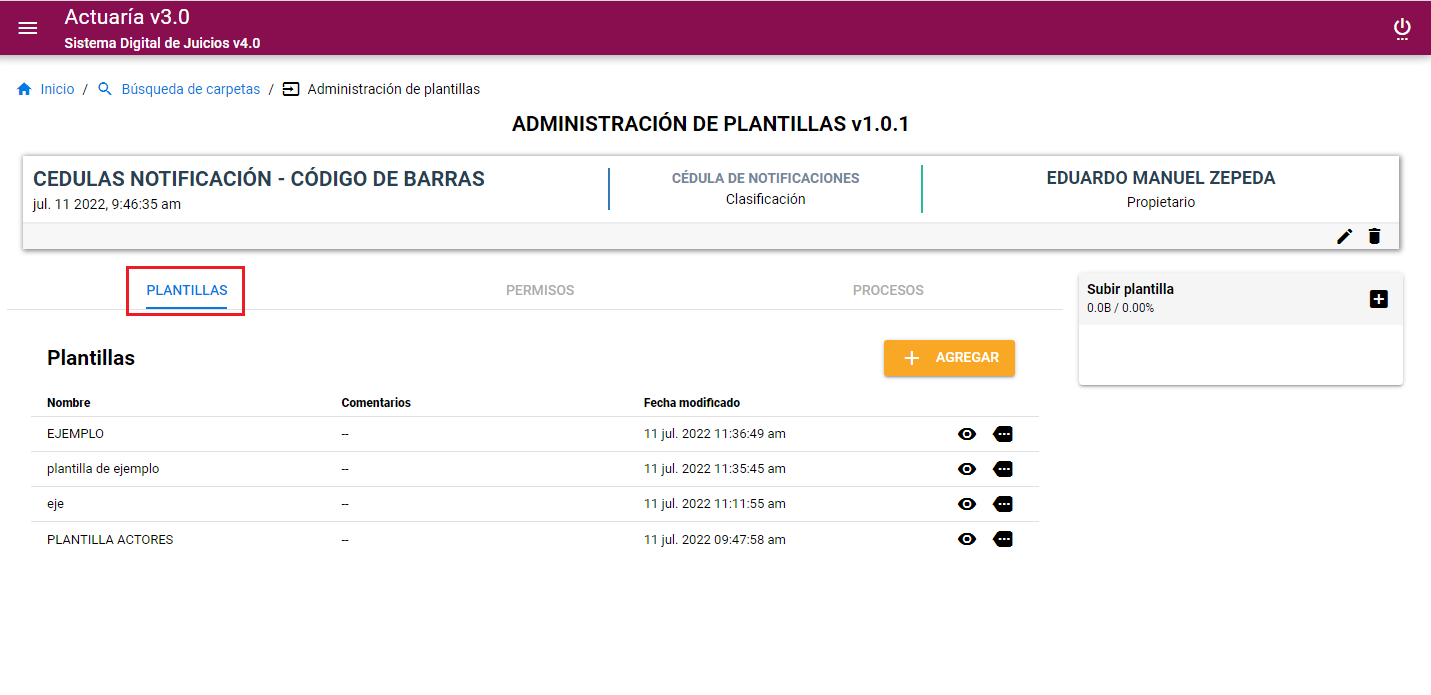
\includegraphics[width=0.90\columnwidth]{adminp.png}
\end{center}

Podemos {\bf{ <<Subir plantilla>>}} dando clic en el botón +

\begin{center}
    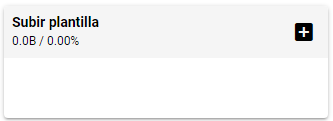
\includegraphics[width=0.50\columnwidth]{subir.png}
\end{center}


Seleccionando desde nuestros archivos la plantilla deseada y damos clic en {\bf{ <<Abrir>>}}

\begin{center}
    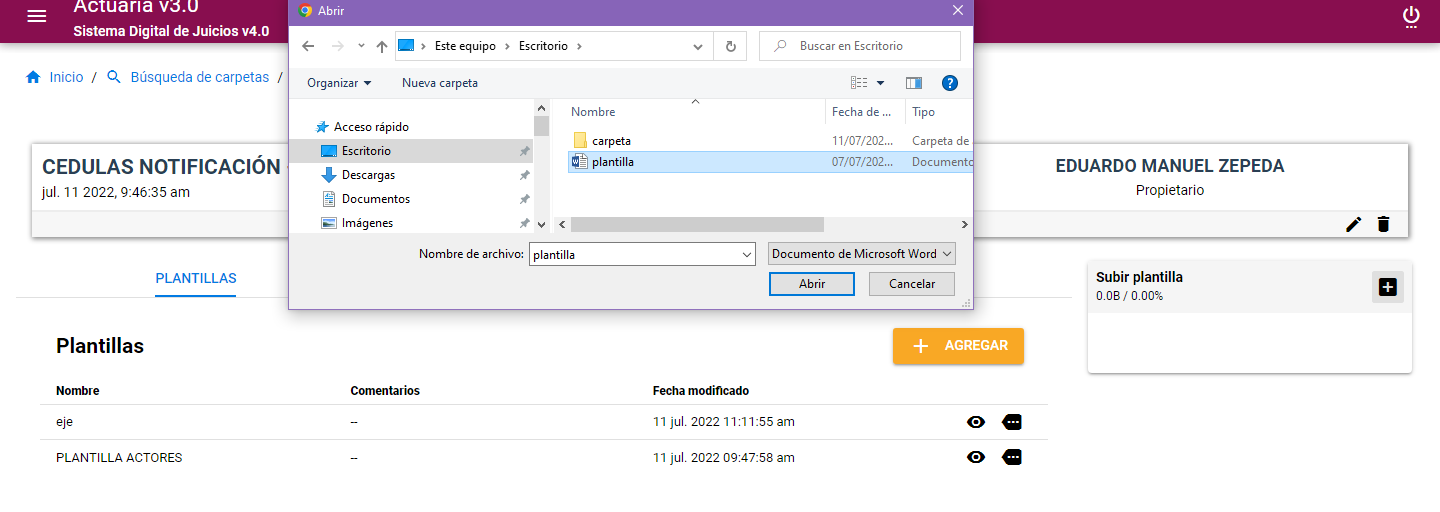
\includegraphics[width=0.90\columnwidth]{plantilla4.png}
\end{center}

Nos aparecerá la siguiente pantalla e ingresaremos los datos de la plantilla y daremos clic en {\bf{ <<GUARDAR>>}}

\begin{center}
    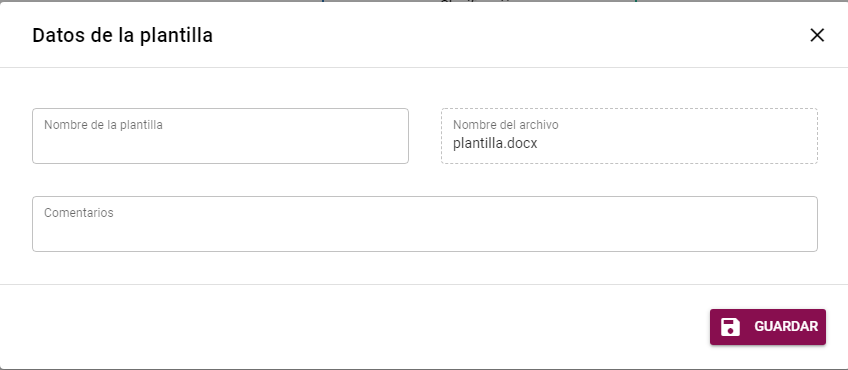
\includegraphics[width=.50\columnwidth]{datosp.png}
\end{center}


De igual forma podemos utilizar el botón 
\includegraphics[width=.15\columnwidth]{agregar.png} para agregar una plantilla.
Dando clic en el nos mostrará la pantalla para ingresar los datos de la plantilla, seleccionar el archivo 
desde nuestros documentos.

\begin{center}
    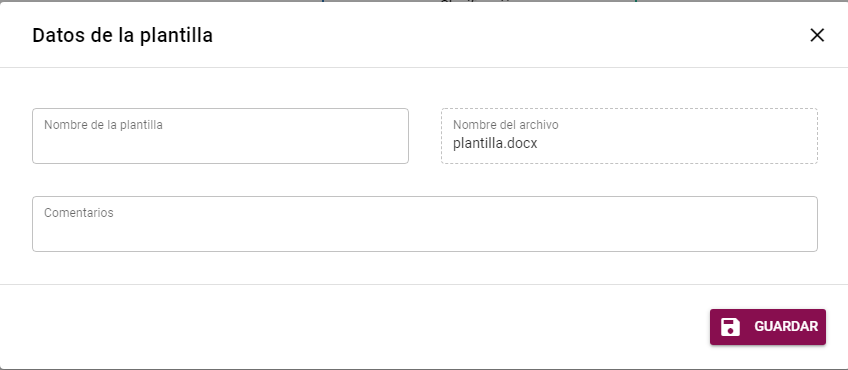
\includegraphics[width=.50\columnwidth]{datosp.png}
\end{center}

A continuación, se enlistan las variables disponibles:

\begin{itemize}
\item \$SALA\$
\item \$PONENCIA\$
\item \$NOJUICIO\$
\item \$ACTUACION\$
\item \$ACTOR\$
\item \$ACTUARIO\$
\item \$AUTORIDADES\$
\item \$TERCEROS\$
\item \$ACTORES\$
\item \$RA\$
\item \$RRC\$
\item \$FECHA\_ELABORACION\_CEDULA\$
\item \$AUTORIZADOS\$
\item \$DOMICILIO\_NOTIFICACIONES\$
\item \$TIPO\_ACUERDO\$
\item \$FECHA\_ACUERDO\$
\end{itemize}

El formato definido en el texto que compone la variable, será respetado por el sistema; por ejemplo,
Negrita, Cursiva y Subrayado:\\
- {{\bf
\$PONENCIA\$ }} \\
\textit{- \$DOMICILIO\_NOTIFICACIONES\$\\}
-\underline{ \$ACTUARIO\$\\}

Ejemplo de cédula:
\begin{center}
    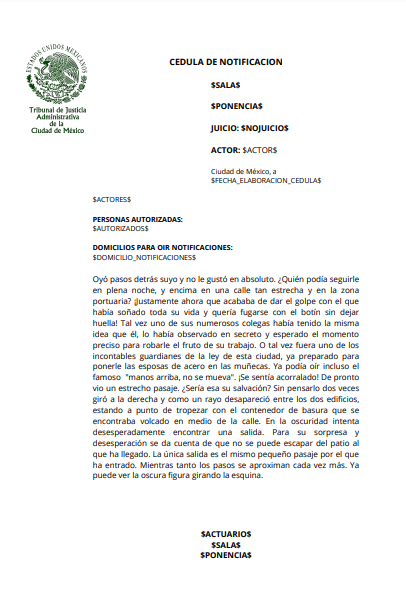
\includegraphics[width=0.80\columnwidth]{cedula.png}
\end{center}

Para cada plantilla podemos realizar las siguientes acciones:
\begin{center}
    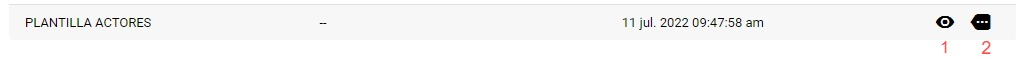
\includegraphics[width=.88\columnwidth]{accionp.jpeg}
\end{center}

\begin{enumerate}[1.]
    \item Visualizar
    \item Más
\end{enumerate}

Para visualizar el documento daremos clic en el icono     
\includegraphics[width=.05\columnwidth]{ojo.png}
Y nos aparecerá nuestra plantilla.
\begin{center}
    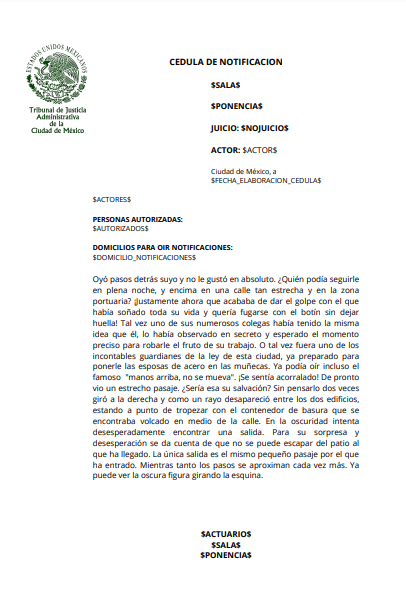
\includegraphics[width=0.55\columnwidth]{cedula.png}
\end{center}

La opción {\bf{ <<Más>>}} nos ofrece lo siguiente:\\
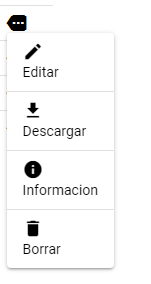
\includegraphics[width=0.20\columnwidth]{mas3.png}

La opción {\bf{ <<Editar>>}} nos permite editar los datos de nuestra plantilla, dando clic en     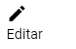
\includegraphics[width=0.10\columnwidth]{edi.png}, nos aparecerá la siguiente pantalla.
\begin{center}
    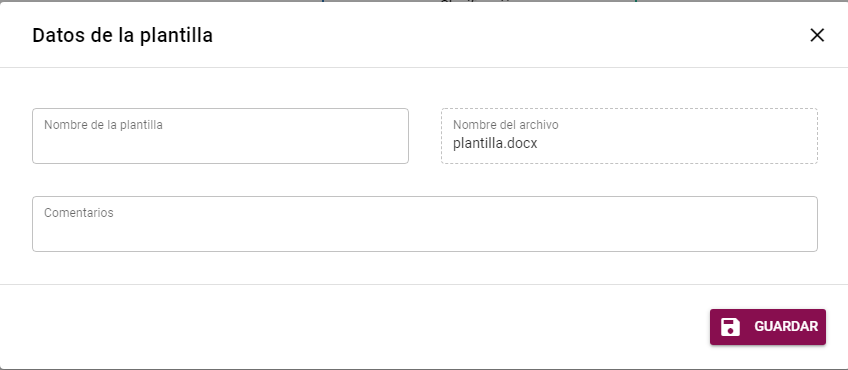
\includegraphics[width=0.50\columnwidth]{datosp.png}
\end{center}

Después de editar nuestros datos deseados daremos clic en el botón {\bf{ <<GUARDAR>>}}
\vspace{1cm}

La opción {\bf{ <<Descargar>>}} nos permite descargar nuestra plantilla y guardarla en nuestro equipo, para hacerlo daremos clic en la opción     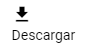
\includegraphics[width=0.10\columnwidth]{desc.png} y seleccionaremos donde queremos que se guarde.
\begin{center}
    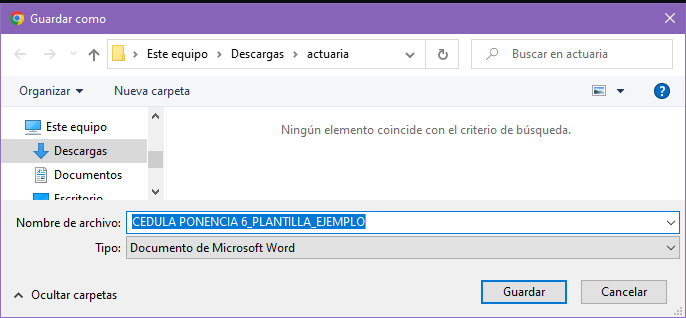
\includegraphics[width=0.60\columnwidth]{descargar.png}
\end{center}

Posteriormente se iniciará la descarga en nuestro equipo.
\begin{center}
    
\includegraphics[width=0.88\columnwidth]{descargar1.png}
\end{center}

La opción {\bf{ <<Información >>}} nos permite ver la información de nuestra plantilla, dando clic en  
\includegraphics[width=0.10\columnwidth]{infor.png} y nos aparecerá la información

\begin{center}
    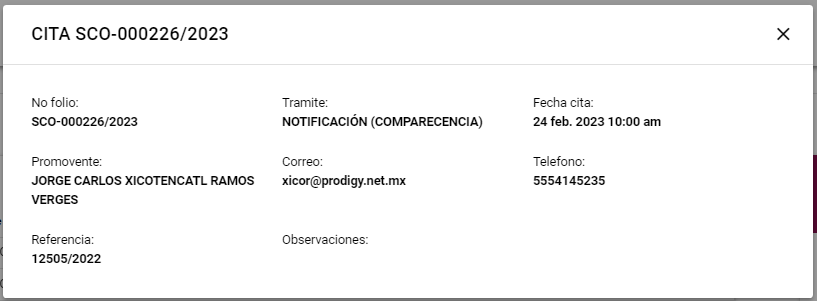
\includegraphics[width=0.8\columnwidth]{inf.png}
\end{center}

Con la opción {\bf{ <<Borrar>>}} podremos borrar nuestra plantilla, dando clic en  en el icono y
nos aparecerá el siguiente mensaje:

\begin{center}
    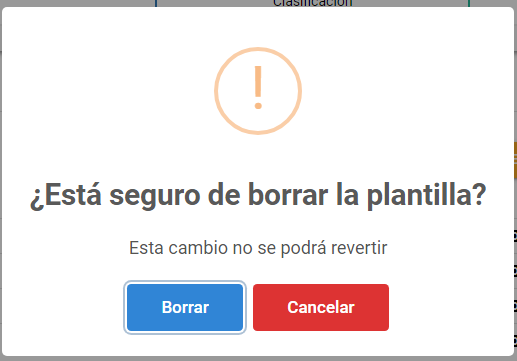
\includegraphics[width=.50\columnwidth]{borrarp.png}
\end{center}

Daremos clic en <<Borrar>>

\vspace{1cm}

En la opción {\bf{ PERMISOS}}

\begin{center}
    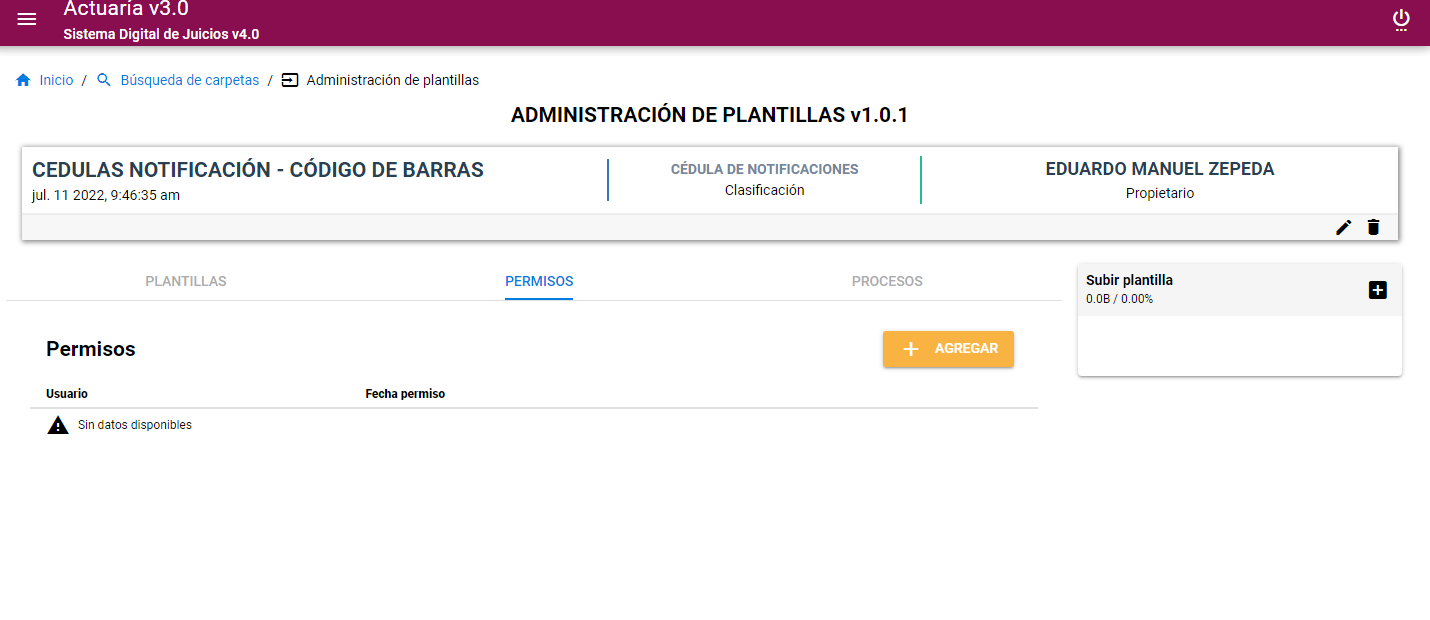
\includegraphics[width=0.88\columnwidth]{permi1.png}
\end{center}

Podemos agregar nuevos permisos, dando clic en el botón     
\includegraphics[width=.15\columnwidth]{agregar.png}, nos aparecerá la siguiente pagina:

\begin{center}
    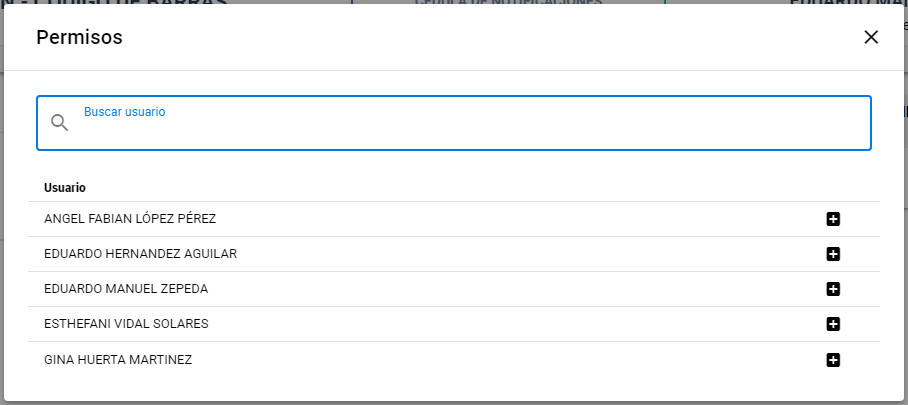
\includegraphics[width=0.88\columnwidth]{permi2.png}
\end{center}

Podemos buscar o seleccionar al usuario con el botón + y automáticamente se agregara mostrando el siguiente mensaje.

\begin{center}
    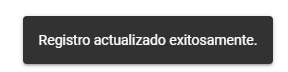
\includegraphics[width=0.30\columnwidth]{permi3.png}
\end{center}

También podemos eliminar el usuario dando clic en el icono     
\includegraphics[width=0.05\columnwidth]{iconob.png}, nos aparecerá el siguiente mensaje:

\begin{center}
    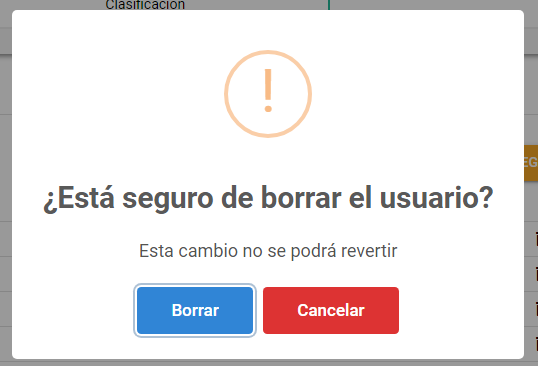
\includegraphics[width=.50\columnwidth]{busuario.png}
\end{center}

Daremos clic en {\bf{ <<Borrar>>.}}
\vspace{1cm}

En la opción {\bf{ PROCESOS}}

\begin{center}
    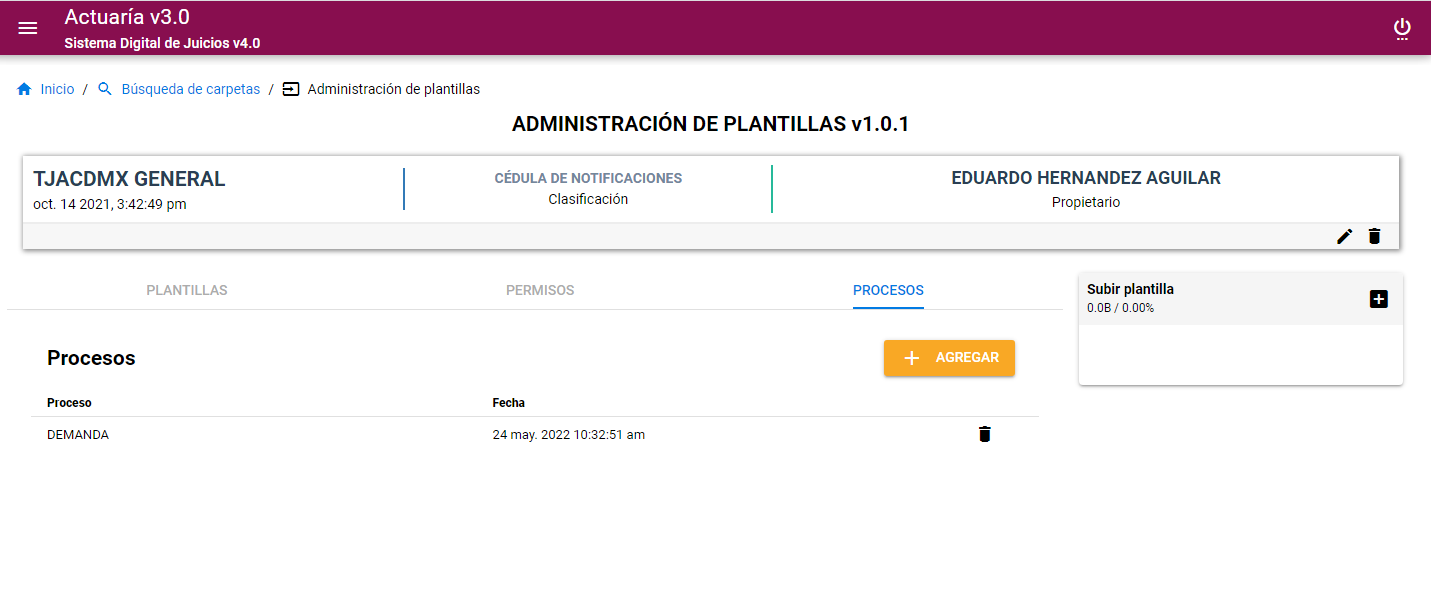
\includegraphics[width=.88\columnwidth]{proc1.png}
\end{center}

Podemos agregar procesos dando clic en el botón   
\includegraphics[width=.15\columnwidth]{agregar.png}, nos aparecerá la siguiente pagina

\begin{center}
    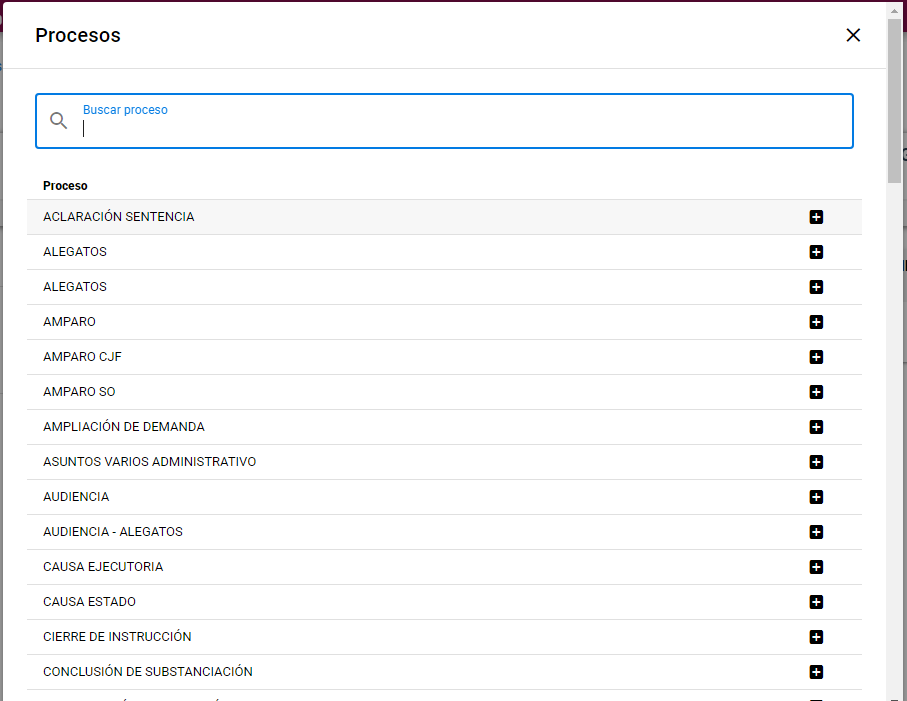
\includegraphics[width=.88\columnwidth]{proc2.png}
\end{center}

Elegiremos los procesos que deseemos dando clic en el +  y automáticamente  se registrara.

\begin{center}
    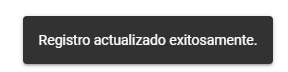
\includegraphics[width=.50\columnwidth]{permi3.png}
\end{center}

Podemos borrar el proceso dando clic en el icono    
\includegraphics[width=.05\columnwidth]{iconob.png} y nos aparecerá el siguiente mensaje

\begin{center}
    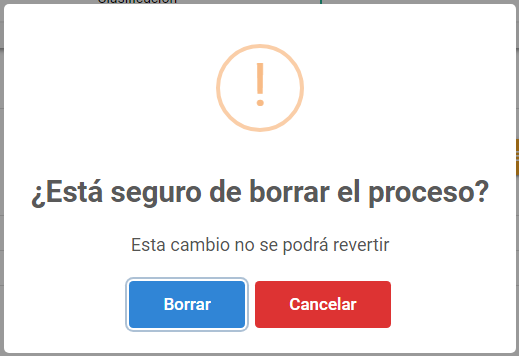
\includegraphics[width=.50\columnwidth]{bproceso.png}
\end{center}

Elegiremos la opción Borrar.
\vspace{1.0 cm}
{{\bf
(2) Añadir plantilla}}
utilizando el icono +

\begin{center}
    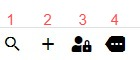
\includegraphics[width=.40\columnwidth]{iconos.jpeg}
\end{center}

Daremos clic en el icono + y nos aparecerá la siguiente pantalla:

\begin{center}
    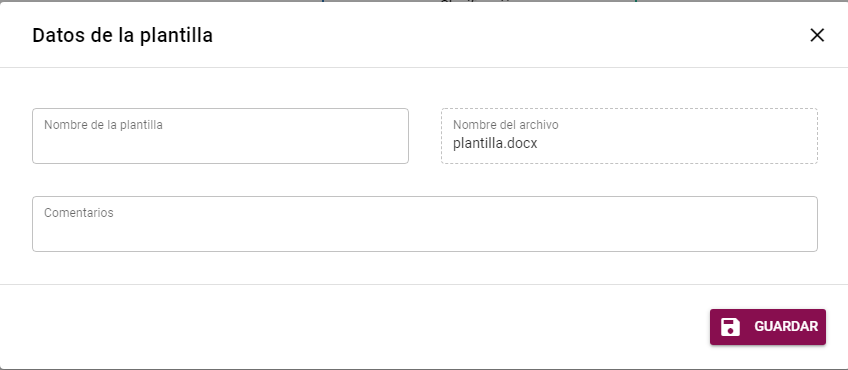
\includegraphics[width=.88\columnwidth]{datosp.png}
\end{center}

Ingresaremos los datos de la plantilla, y seleccionaremos
el archivo desde nuestros documentos.

\begin{center}
    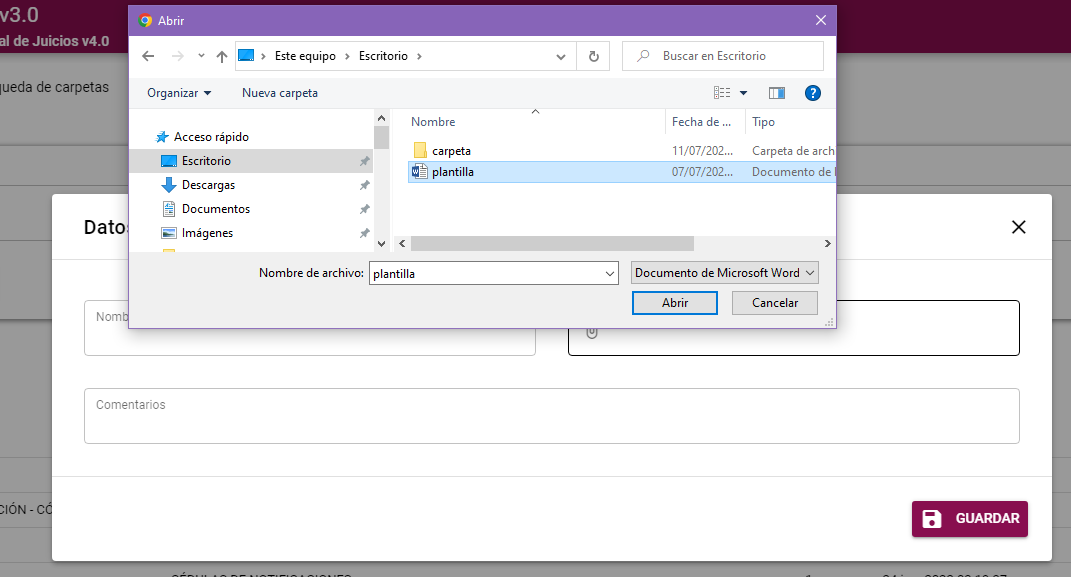
\includegraphics[width=.88\columnwidth]{plantilla10.png}
\end{center}

Daremos clic en <<Abrir>> , el sistema agregara el archivo y daremos clic en el botón  {{\bf
<<GUARDAR>>}}


{{\bf (3) Agregar permisos}}\\
Daremos clic en el icono     
\includegraphics[width=.05\columnwidth]{permisos2.png}
y nos aparecerá la siguiente pantalla:

\begin{center}
    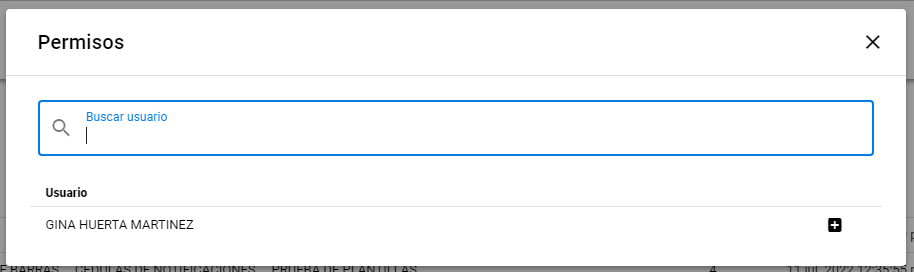
\includegraphics[width=.88\columnwidth]{permi6.png}
\end{center}

Seleccionares la opción deseada con el icono +
Y automáticamente se registrara en el sistema, mostrado el siguiente mensaje.

\begin{center}
    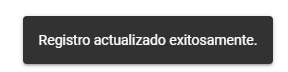
\includegraphics[width=.30\columnwidth]{permi3.png}
\end{center}

Ingresaremos los datos de la plantilla, y seleccionaremos
el archivo desde nuestros documentos.

{{\bf (4) Más}}\\El icono

\includegraphics[width=.05\columnwidth]{mas2.png}
nos ofrece  las siguientes opciones:

\begin{center}
    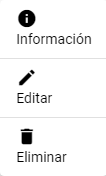
\includegraphics[width=.15\columnwidth]{mas10.png}
\end{center}

La opción     
\includegraphics[width=.10\columnwidth]{infor.png}
nos permite ver la información de la carpeta
dando clic .

\begin{center}
    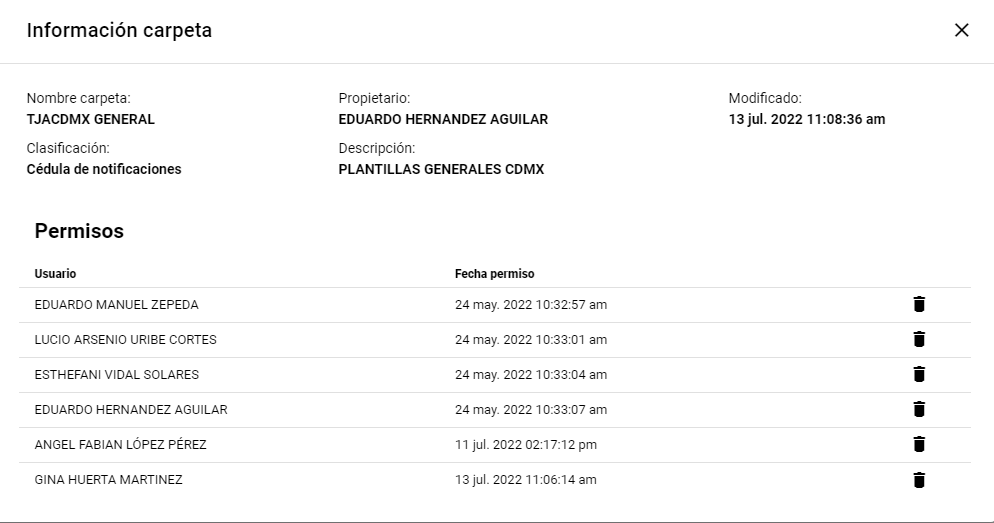
\includegraphics[width=.88\columnwidth]{incarpeta.png}
\end{center}

Podemos ver:
\begin{itemize}
    \item Nombre carpeta
    \item Propietario
    \item Modificación
    \item Clasificación
    \item Descripción
    \item Permisos
\end{itemize}

Y oportunidad de borrar permisos dando clic en el icono

\includegraphics[width=.05\columnwidth]{iconob.png}\\
La opción     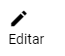
\includegraphics[width=.10\columnwidth]{editar10.png}
nos permite editar el grupo.
Para ello daremos clic y nos aparecerá la siguiente pantalla:

\begin{center}
    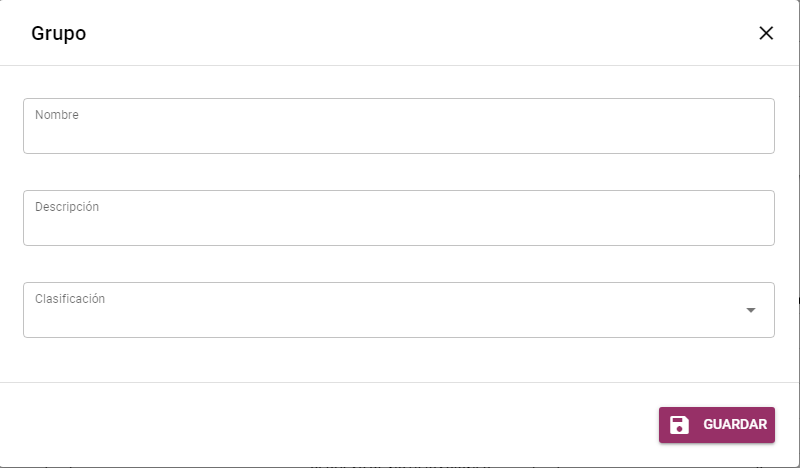
\includegraphics[width=.50\columnwidth]{GRUPO.png}
\end{center}

Podemos editar:
\begin{itemize}
    \item Nombre
    \item Descripción
    \item Clasificación
\end{itemize}

Después de editar lo deseado daremos clic en el botón {{\bf
<<GUARDAR>>}}

La opción     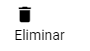
\includegraphics[width=.10\columnwidth]{eliminar.png}
nos permite eliminar el grupo.\\
Para ello daremos clic y nos aparecerá el siguiente mensaje:

\begin{center}
    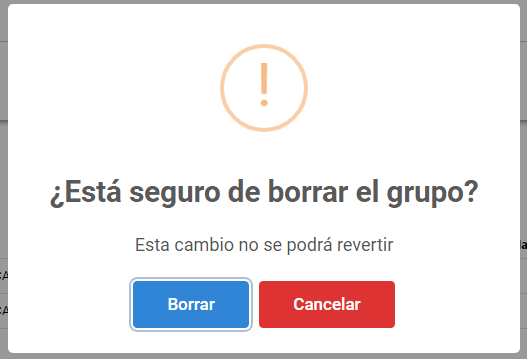
\includegraphics[width=.50\columnwidth]{eligrupo.png}
\end{center}

Daremos clic en el botón {\bf{<<Borrar>>}}

\chapter{\large{Administración de Leyendas v1.0.0}}\label{chap:leyendas}
En este módulo podemos:
\begin{enumerate}[(1)]
    \item Buscar leyenda
    \item Registrar leyenda
    \item Editar leyenda
    \item Borrar leyenda
\end{enumerate}

\begin{center}
    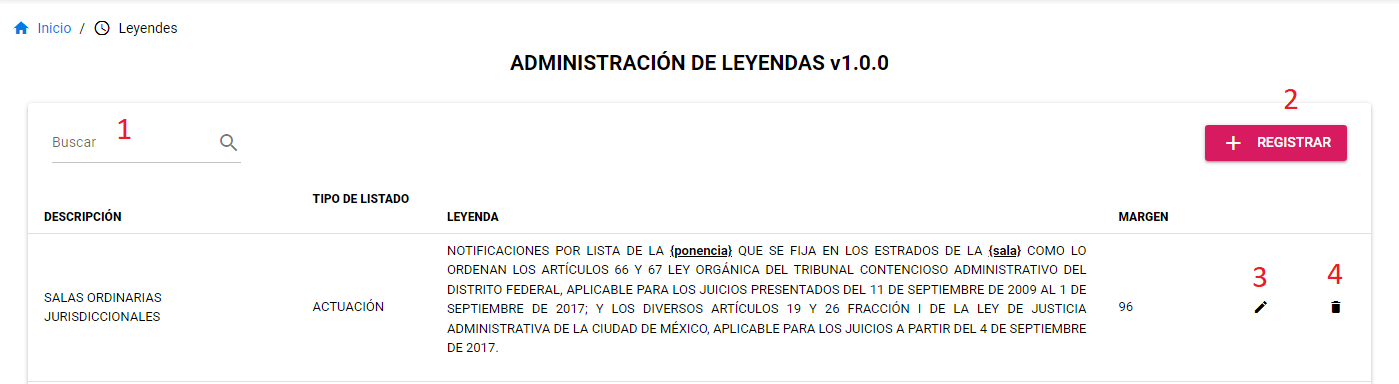
\includegraphics[width=0.90\columnwidth]{leyendas.png}
\end{center}

{\Huge{\color{myblue} \section{Buscar leyenda}\label{sec:28}}}

Para buscar una leyenda bastará con ingresar el texto en el buscador que se encuentra de lado superior izquierdo, identificado con el número 1.  \textit{Ver ~\nameref{chap:leyendas}}\\

{\Huge{\color{myblue} \section{ Registrar leyenda}\label{sec:29}}}

Para registrar una leyenda de clic sobre el botón {\bf{<<REGISTRAR>>}}
se mostrará una pantalla con los siguientes datos.

\begin{center}
    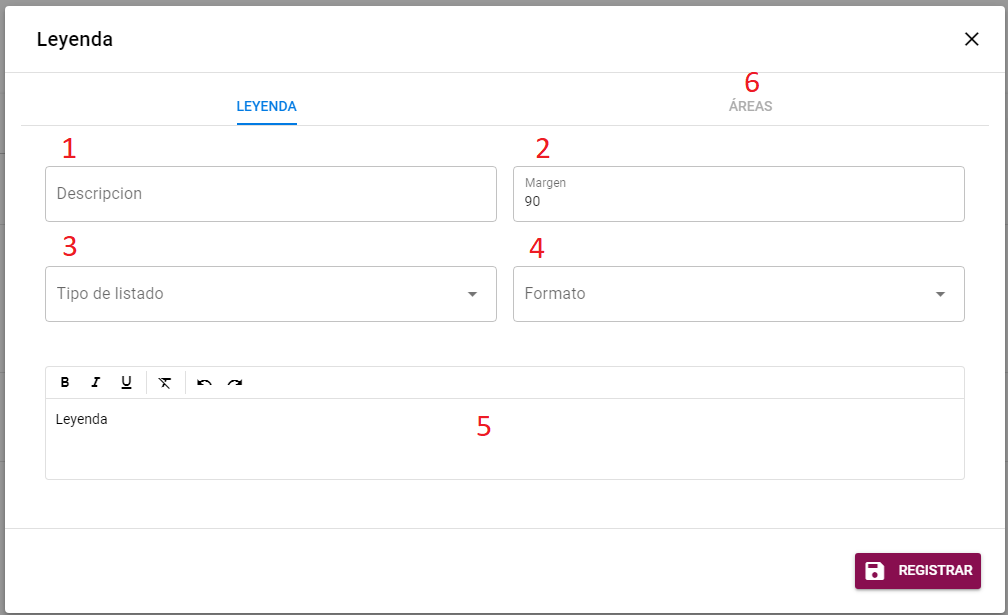
\includegraphics[width=0.77\columnwidth]{leyenda_datos.png}
\end{center}

Ingresa:
\begin{enumerate}
    \item Descripción
    \item Margen
    \item Tipo de listado
    \item Formato
    \item Leyenda
    \item Áreas
\end{enumerate}

Posteriormente da clic en el botón {\bf{<<GUARDAR>>}}

{\Huge{\color{myblue} \section{Editar leyenda}\label{sec:30}}}

Para editar una leyenda bastará con dar clic sobre el icono {\bf{ <<Editar>>}} que se encuentra de lado derecho, identificado con el número 3   \textit{Ver ~\nameref{chap:leyendas}}\\
Edite los datos deseados y de clic en el botón actualizar

\begin{center}
    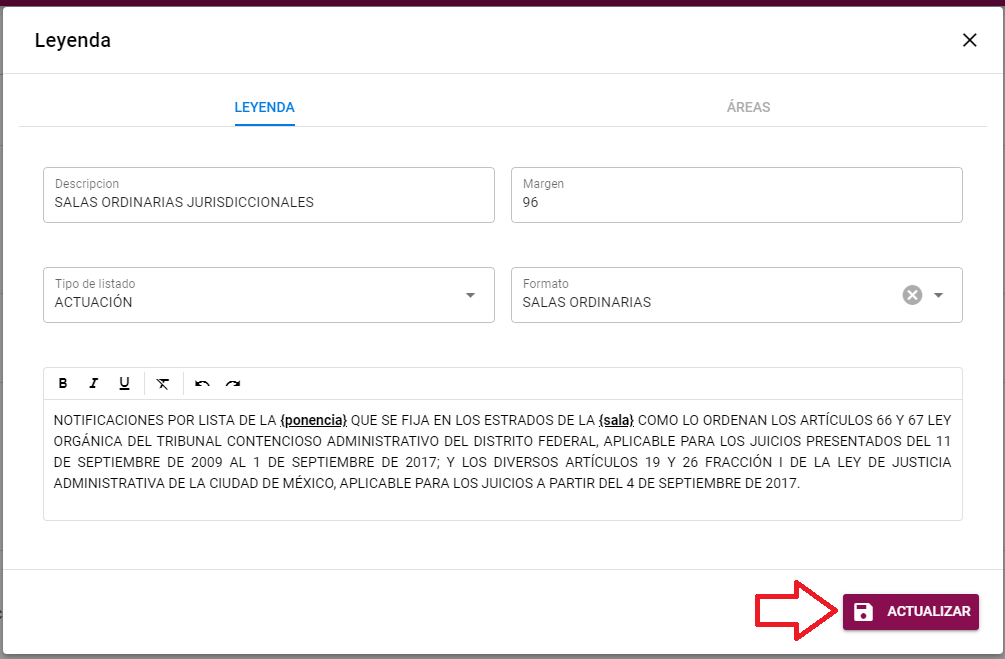
\includegraphics[width=0.77\columnwidth]{actualizar.png}
\end{center}


{\Huge{\color{myblue} \section{Borrar leyenda}\label{sec:30.1}}}

Para borrar una leyenda bastará con dar clic sobre el icono {\bf{ <<Borrar>>}} que se encuentra de lado derecho, identificado con el número 4   \textit{Ver ~\nameref{chap:leyendas}}\\
Se mostrará un mensaje de advertencia, da clic en el botón aceptar.


\begin{center}
    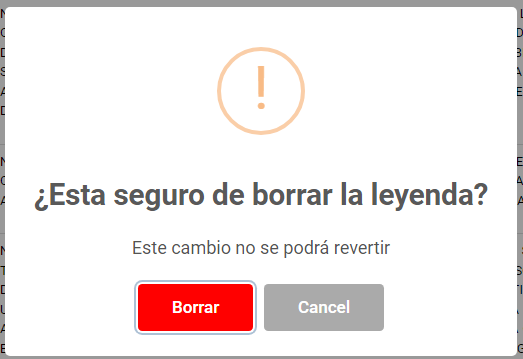
\includegraphics[width=0.44\columnwidth]{borrar.png}
\end{center}

\newpage
\begin{table}[t]
\begin{center}
\begin{tabular}{| c | c | c | c | }
\hline

\multicolumn{4}{ |c| }{\cellcolor[gray]{0.9}CONTROL DE VERSIONES} \\ \hline
Versión &               Elaborado por:          & Fecha de última modificación          & Motivo \\ \hline
1.0.1   & Esthefania Vidal Solares        &      12/octubre/2022
&Creación \\ \hline
1.0.2   & Esthefania Vidal Solares        &     27/febrero/2023
&Actualización \\ \hline
\hline
\end{tabular}
\caption{Control de Versiones}
\label{tab:versiones}
\end{center}
\end{table}

\end{quote}

\end{document}